\subsection{Инверсия зависимостей}

Принцип инверсии зависимостей -— важный принцип объектно-ориентированного программирования, используемый для уменьшения зацепления в компьютерных программах. Входит в пятёрку принципов SOLID и строится из двух правил:
\begin{itemize}
	\item модули верхних уровней не должны зависеть от модулей нижних уровней. Оба типа модулей должны зависеть от абстракций;
	\item абстракции не должны зависеть от деталей. Детали должны зависеть от абстракций.
\end{itemize}

До появления безопасного в использовании полиморфизма, многие програмы выглядели следующим образом: высокоуровневые функции вызывали функции уровнем ниже, те, в свою очередь, вызывали функции ещё ниже и так продолжая. Таким образом, зависимости в коде диктовались потоком управления. На Рисунке \ref{img:direct:dep} изображен пример графа связанности модулей, на который наложен поток выполнения в ситуации, когда не применяется инверсия зависимостей.

\begin{figure}[h]
  \centering
    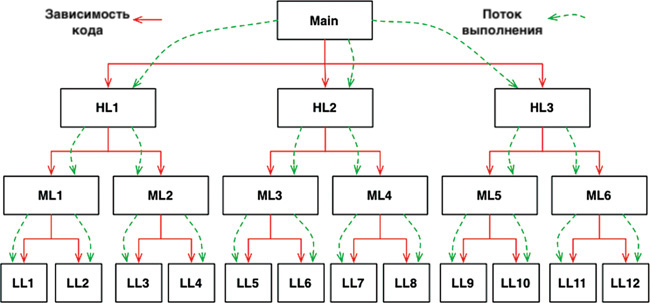
\includegraphics[width=0.8\textwidth]{inc/img/direct.jpeg}
    \caption{Прямые зависимости}
  \label{img:direct:dep}
\end{figure}

Что б функция \lstinline[language=C]{main()} вызвала любую из высокоуровневых функций(HL1, HL2, HL3), разработчику придётся сделать зависимость на модуль, в котором эта функция объявлена(написав конструкцию \lstinline[language=C]{#include}). Вызывающий обязан связываться с модулем, в котором находится вызываемый.

Такое требование сильно связывает руки проектировщикам: поток управления диктуется поведением системы, а зависимости в коде -- потоком управления. С применением полиморфизма можно добиться совершенно иного результата, показанного на изображении \ref{img:inverted}. Модуль HL1 вызывает функцию F() в модуле ML1, при этом не имея на него зависимости.

\begin{figure}[h]
	\centering
	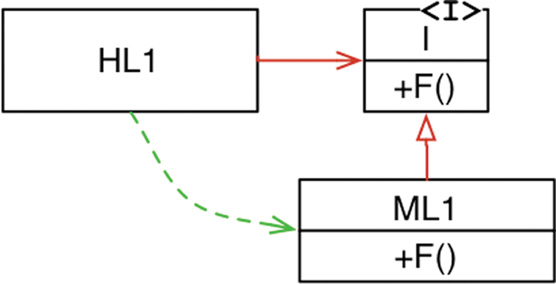
\includegraphics{inc/img/inverted.jpeg}
	\caption{Инвертированная зависимость}
	\label{img:inverted}
\end{figure}

Подобный инструмент позволяет, например, заставить слой базы и пользовательского интерфейса зависеть от бизнес логики, хоть поток управления и идёт в другую сторону. Подобные изменения позволят заменять базу без каких-либо изменений в бизнес логике. Выпускать компонент с бизнес логикой без пользовательского интерфейса.
